\documentclass{njureport}

\begin{document}
\makecover
\pagestyle{plain}
\part{数值方法求解定积分:用不同求积方法计算定积分值}

\section{题干}
  \textbf{用不同积分方法计算如下定积分值}
    $$\int _0^1\sqrt{x}\ln{x} \,dx$$

  \begin{description}[itemindent=1em]
  \item[算法1]    取不同的步长\emph{h}。分别用复化梯形及复化辛普森求积公式计算积分,
  \item[算法2]    用龙贝格求积计算完成问题1,使其精度达到\textcolor{red}{$10^{-4}$}。
  \end{description}
\section{分析}
 \begin{description}[itemindent=1em]
  \item[算法1] 取不同步长,使用{\textcolor{blue}{复化梯形}}及{\textcolor{blue}{复化辛普森求积公式}}计算定积分值.
  \item[算法2] 总结一下,可以得到龙贝格算法的过程如下:

$$
    \left\{\begin{array}{lcl}
     T_1=\dfrac{b-a}{2}[f(a)+f(b)]\\[1em]
     T_{2^k}=\dfrac{1}{2}T_{2^{k-1}}+\dfrac{b-a}{2^k} \sum_{j=0}^{2^{k-1}-1}f(a+(2j+1)\dfrac{b-a}{2^k})\quad k=1,2,\ldots\\[1em]
     S_{2^{k-1}}=\dfrac{4}{3}T_{2^k}-\dfrac{1}{3}T_{2^{k-1}}\\[1em]
     C_{2^{k-1}}=\dfrac{16}{15}S_{2^k}-\dfrac{1}{15}S_{2^{k-1}}\\[1em]
     R_{2^{k-1}}=\dfrac{64}{63}C_{2^k}-\dfrac{1}{63}C_{2^{k-1}}\\[1em]
     T_{m+1}(h)=\dfrac{4^mT_m(h/2)}{4^m-1}-\dfrac{T_m(h)}{4^m-1}
    \end{array}\right.$$
    其中$T_m(h)$指步长为\emph{h}的\emph{2m-2}阶\emph{Newton-Cotes}公式计算结果,$T_m(\dfrac{h}2)$ 指步长为${\dfrac{h}2}$的\emph{2m-2}阶\emph{Newton-Cotes}公式计算结果。
 \end{description}

\section{程序流程图}
随便来张图:
\begin{figure}[H]
 \center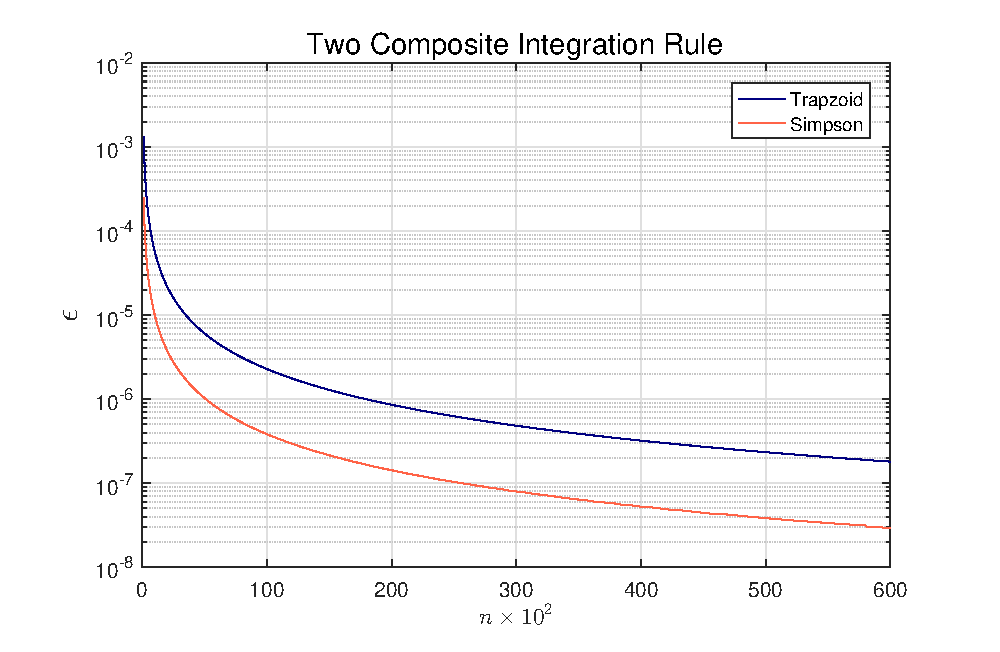
\includegraphics[width=\textwidth]{material/6_1_e.eps}
 \caption{\textrm{用复化梯形及复化辛普森求积公式计算积分}}
 \end{figure}

\section{运行结果}
    $0\neq1$
\section{结果分析}
\begin{description}[itemindent=1em]
  \item[算法1] 探究复化求积公式的误差,根据其余项公式可得到:

    \textbf{复化梯形公式}的余项是区间步长\textit{h}的2阶无穷小量:
     $$R_n(f)=-\dfrac{b-a}{12}h^2f''(\eta)\quad\eta\in[0,1]$$
  \item[算法2] 龙贝格求积方法可总结为$$T_{m+1}(h)=\dfrac{4^mT_m(h/2)}{4^m-1}-\dfrac{T_m(h)}{4^m-1}$$
    其中$T_m(h)$指步长为\emph{h}的\emph{2m-2}阶\emph{Newton-Cotes}公式计算结果,$T_m(\dfrac{h}2)$ 指步长为${\dfrac{h}2}$的\emph{2m-2}阶\emph{Newton-Cotes}公式计算结果。在实际计算中,一直计算到$|T_{m+1}(h)-T_m(h)|<\varepsilon=1\times10^{-4}$为止。

    采用这种计算方法,可得到$m=4$,龙贝格积分值为\textcolor[rgb]{1.00,0.00,0.00}{$-0.43760383679$};若采用$|R-I|<\varepsilon=1\times10^{-4}$ 为终止计算条件,可以得到不同的结果:$m=9$,龙贝格积分值为\textcolor[rgb]{1.00,0.00,0.00}{$-0.44438622012$}.
\end{description}
\section{编程总结}
\begin{enumerate}[1.]
  \item 处理数据时,可简单定义一个量以量化指示某种需要观察得到的变化,可通过编程简单计算再结合画图直观呈现的方式获得更好的理解。
  \item 递归函数难度较大,常需要结合分治的思想,但一些可以借用循环完成的过程,不必要引入递归函数的操作
\end{enumerate}

\section{源代码}
 \lstinputlisting{material/code.f90}

\end{document}
